\chapter{Results and discussion}\label{ch:results}
%%%%%%%%%%%%%%%%
%- Introduction of what we are looking for, reminder of hypothesis
%%%%%%%%%%%%%%%%
This chapter discusses the experimental data pursuing the hypothesis that tampered layer around nanometer sized single particles inhibit the radiation damage process. To verify this hypothesis, we will first investigate the radiation damage in pristine Xe-cluster using the data from the described pump--probe experiment in section \ref{sec:xenon-data}. After having clarified the X-ray induced effects in Xe-cluster, we continue to discuss the heterogeneous data of the HeXe-cluster in section \ref{sec:helium-data}, while comparing it to the pristine He-data. Alongside this discussion, we will make use of the methods described in the previous chapter \ref{ch:methods}.
%
%
%
%%%
\section{Pristine xenon pump--probe diffraction images}\label{sec:xenon-data}
%%%%%%%%%%%%%%%%%%%%%%%%%%%
%- Presentation of Xe data
%%%%%%%%%%%%%%%%%%%%%%%%%%%
% INTRO
A large scale analysis of size, shape and other parameter has been performed on single-shot diffraction patterns of xenon cluster to investigate the nanoplasma transition. Thereby a X-ray pump pulse starts X-ray induced effects, i.e. the nanoplasma transition and a X-ray probe pulse at a later time $\Delta t$ enables us to take a snapshot of the system.\\
The analysis starts by selecting hits from non-hits using the methods described in section \ref{sec:hitfinding}. Using these filters, a typical run length per delay time is 20 mins, i.e. $\sim 144,000$ images. These events are automated reduced to $\sim 1000$ events and then semi-automated reduced to a subset of 30 - 60 single-shot diffraction patterns per delay setting. This breakdown further allows the estimation that $0.02\% - 0.04\%$ of all imaged xenon cluster had good parameter for analysis. This figure is likely understating the amount of analyzable hits, however, this selection includes the events that show a nanoplasma transition but are still suitable for phase-retrieval (compare figure \ref{fig:filter-size-intensity}).\\
% SIZE EFFECTS
\begin{figure}
	\centering
		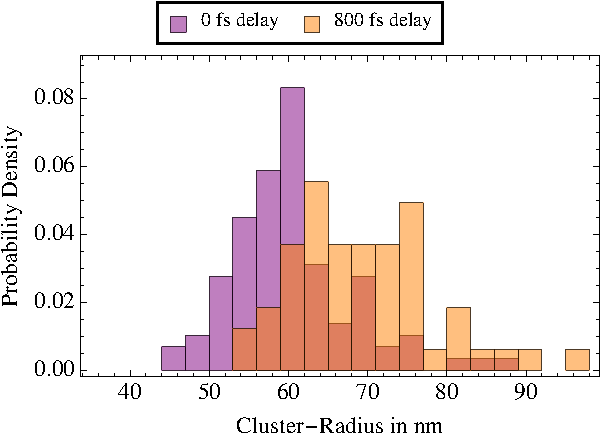
\includegraphics[width=0.75\textwidth]{images/size-distributions.pdf}
	\caption{Size evaluation of $\sim 30$ single Xe-cluster hits per time delay $\Delta t$ step. At $\Delta t=0$ fs, the size distribution follows an expected log-normal distribution, while at $\Delta t=800$ fs the distribution broadens and shifts towards larger radii due to the nanoplasma transition.}
	\label{fig:size-distributions}
\end{figure}
Figure \ref{fig:size-distributions} shows a distribution of sizes at the pump--probe delays $\Delta t = \left\{0,800\right\}$ fs. Here, equation \eqref{eq:scattering from sphere} has be abused to semi-automate the size determination process to enable the high-throughput size evaluation. The size distribution of Xe-cluster follows a log-normal distribution \citep{Schutte-2002-IJMS} and at $\Delta t=0$ fs the mean cluster radius is 61 nm. When the delay is increased to $\Delta t=800$ fs, the mean cluster radius increases to 74 nm. Additionally, the distribution becomes more broad, which is due to the varying pump-pulse strength. Over the course of 800 fs, the nanoplasma transition drives an expansion of the cluster that is on average $\sim 20 \%$. Figure \ref{fig:filter-size-intensity} left shows that the expansion speed is constant and summarizes the mean cluster radii over the pump--probe delay steps $\Delta t=\{0,120,250,400,800\}$. From here, we can estimate the electron temperature of the nanoplasma. It is assumed that electrons thermalize with the nucleus within a few femtoseconds such that the mean velocity of the hot electron gas follows a Maxwell-Boltzmann distribution. If we use the average expansion speed $\sim 15250$ m/s as mean velocity of a Maxwell-Boltzmann distribution the electron temperature is determined to be $\sim 125$ eV. We can compare the electron temperature to a similar IR pump -- X-ray probe study \citep{Gorkhover-2016-NatPho}, where electron temperatures of $\sim 200$ eV have been estimated. This also explains the fast expansion speed in this optical pump--probe study. For the sake of completeness, the IR pump laser had power densities of only $\sim 10^{15}$ W cm$^{-2}$ compared to the $\sim 10^{17}$ W cm$^{-2}$ of the X-ray pump laser in this study but the smaller X-ray absorption cross-sections explain the difference in total absorbed energy from the pump pulse.\\
% NO OF SCATTERER
\begin{figure}
	\centering
		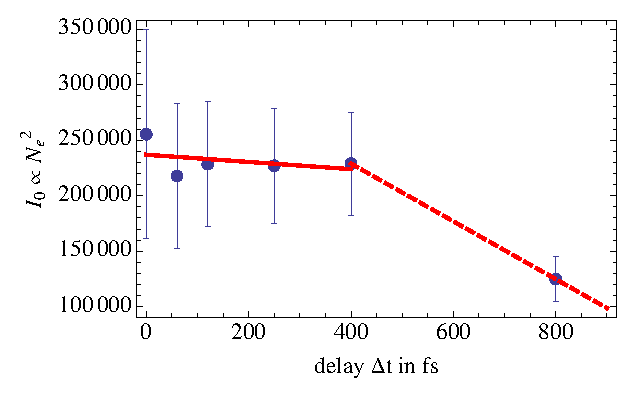
\includegraphics[width=0.80\textwidth]{images/results/number-of-scatterer.eps}
	\caption{Intensity $I$ in arb. units at $\vec{Q}\rightarrow 0$, which is proportional to the total amount of scatterer squared $N_{e}^{2}$, here electrons. The data show that the expanding cluster Coulomb traps electrons steadily in the initial stages of the nanoplasma expansion but as the trapping potential decreases due to the multistep ionization a sudden decrease of $\sim 65\%$ electrons is observed.}
	\label{fig:number-of-scatterer}
\end{figure}
The total number of scatterers, i.e. electrons that interact with LCLS, was deducted from the diffraction patterns as well. As described in the theory section \ref{sec:saxs}, when
\begin{equation}
I\left(\vec{Q}\rightarrow 0\right)\propto N_{e}^{2},
\label{eq:}
\end{equation}
with the scattered intensity $I$ as a function of the scattering vector $\vec{Q}$ and number of electrons that contribute to the scattering process $N_{e}$. Figure \ref{fig:number-of-scatterer} shows the average fitting parameter $I_{0}$, from equation \eqref{eq:scattered-intensity} and \eqref{eq:scattering from sphere}, as a function of the time delay $\Delta t$ (blue dots). Two linear fits (red lines) have been added to the graph to visualize the effect. The averages were obtained in the analysis of $\sim 15-30$ single xenon cluster diffraction pattern per delay step. The data show that up to a delay of $\Delta t=400$ fs the amount of electrons $N_{e}$ in the cluster remains rather constant. However, at a time delay of $\Delta t=800$ fs, the amount of scattering electrons decreased on average by $\sim 26 \%$. This confirms that Coulomb trapping\index{nanoplasma expansion!Coulomb trapping} efficiently traps electrons from the ionization process in the initial stages of the nanoplasma expansion\index{nanoplasma!expansion}, here up to 400 fs after the pump pulse, but eventually the electrons overcome the trapping potential dissipate the interaction region such that they do not contribute to the diffraction image anymore. The key drivers that lower the trapping potential, thus releasing the electrons, is the expansion of the cluster and the progressing multistep ionization. The concept of radiation damage including trapped electrons has been simulated in \citep{Hau-Riege-2004-PRE}, where trapped electrons dominate the damage process due to secondary collisional ionization. Let us now perform a thought-experiment in which a CDI is performed using long X-ray pulses of 100 fs (or so). In such an experiment, electrons would get ionized and trapped efficiently by the Coulomb potential, as the cluster has not yet expanded significantly. During the X-ray pulse duration, multistep ionization increases the ionization level significantly and thus the amount of quasi-free electrons. Now, the trapped electrons in the nanoplasma can be treated non-relativistic, thus they do contribute (coherently) to the scattering pattern. But their contributions blur the effective shape of the imaged object and one has to keep in mind that this comes on top of the actual sample damage, for example broken bonds or further shape changes. A similar electronic damage of a sample is described in \citep{Quiney-2010-NatPhys} and that computational methods may compensate for such damage.\\
% SINGLE SHOT DIFF PATTERN
\begin{figure}
	\centering
		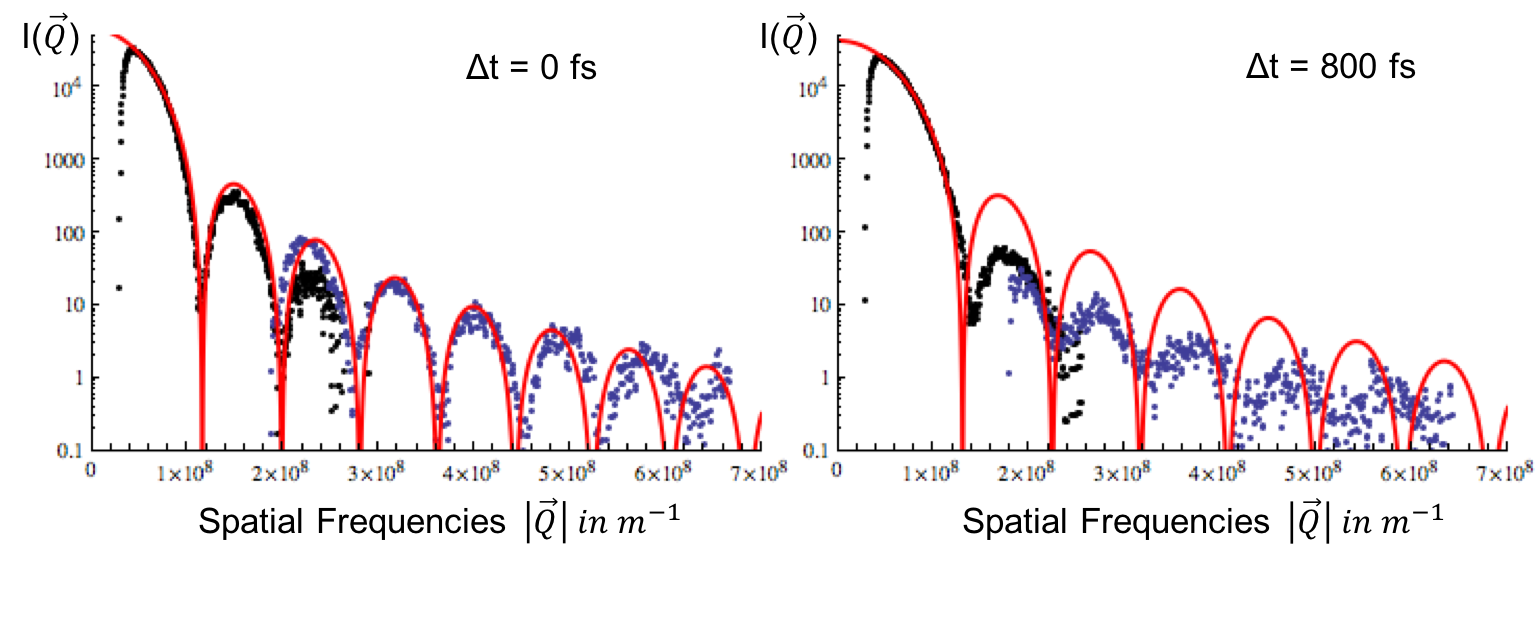
\includegraphics[width=1.0\textwidth]{images/results/Xe-diff-pattern.png}
		%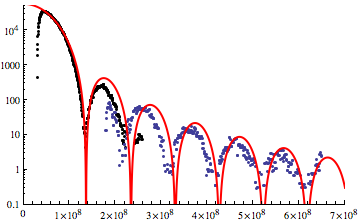
\includegraphics[width=0.49\textwidth]{images/results/Xe-only-60fs.png}\\
		%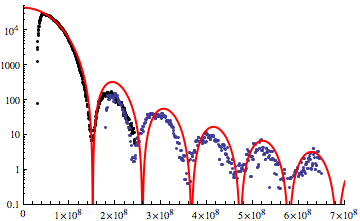
\includegraphics[width=0.49\textwidth]{images/results/Xe-only-120fs.png}
		%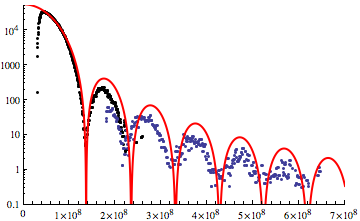
\includegraphics[width=0.49\textwidth]{images/results/Xe-only-250fs.png}\\
		%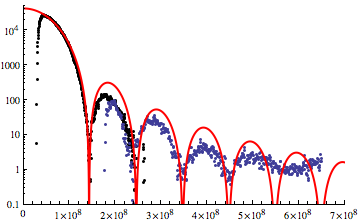
\includegraphics[width=0.49\textwidth]{images/results/Xe-only-400fs.png}
		%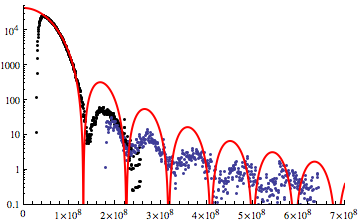
\includegraphics[width=0.49\textwidth]{images/results/Xe-only-800fs.png}
	\caption{Single shot diffraction pattern at certain pump--probe delays $\Delta t$. The red curve simulates the scattering of a sphere, the black data points are from the rear pnCCD detector and the blue data points are from the front pnCCD. The nanoplasma expansion manifests in the scattering intensity $I$ at large spatial frequencies $\vec{Q}$, where $I$ decreases as described in \citep{Gorkhover-2016-NatPho}.}
	\label{fig:Xe-only-diff-pattern}
\end{figure}
Single-shot diffraction pattern 1D projections can be found in figure \ref{fig:Xe-only-diff-pattern}. The figure shows a red line, which is the scattering from a sphere as per equation \eqref{eq:scattered-intensity} and \eqref{eq:scattering from sphere} fitted onto the low-$\vec{Q}$ signal of the zeroth diffraction scattering order using the radius variable and the incident beam intensity. The black data points are projected from the rear pnCCD, the blue data points are projected from the front pnCCD using the projection method described in \ref{sec:combination-of-images}. At $\Delta t=0$ fs, the scattering of the Xe-cluster can be well approximated with the scattering of a sphere and the fit (red line) agrees well with the data points up to scattering angles of $\Theta \approx 9$°. As the time delay $\Delta t$ increases, the large-$\vec{Q}$ scattering signal decreases and the scattering of a plain sphere does not well fit the scattering here. A similar effect is also observed in the previously mentioned IR pump--probe study \citep{Gorkhover-2016-NatPho}. Due to the nanoplasma transitions the Xe-cluster is expanding with the outer layers expanding faster than the core as it is described in, e.g. \citep{Hau-Riege-2004-PRE}. A similar damage model has been introduced in section \ref{sec:2d-simulations} and generally fits the data well. This is shown in great detail in \citep{Gorkhover-2016-NatPho,Gorkhover-2014-Thesis}. Note that the pump--probe considerations from section \ref{sec:pump--probe-considerations} would minimize the effect of a decreased scattering a large scattering angles.\\
% 1D RECONSTRUCTIONS
\begin{figure}
	\centering
		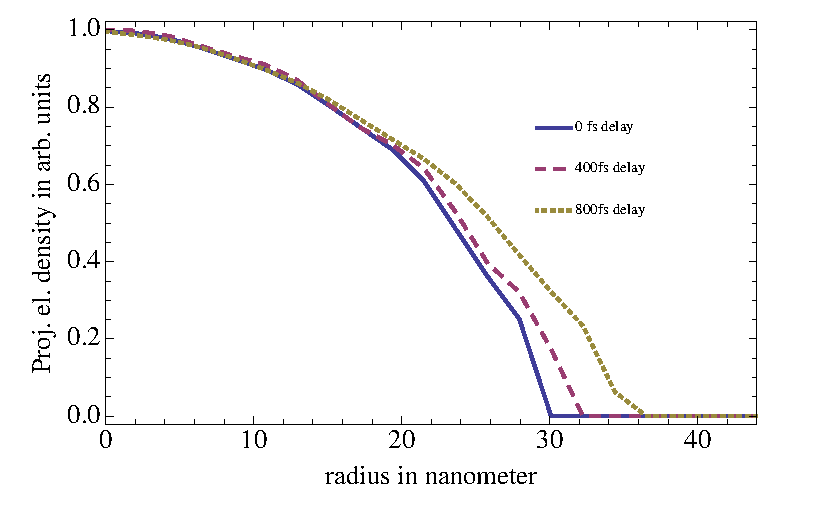
\includegraphics[width=0.80\textwidth]{images/results/Xe-reconstructions.eps}
	\caption{Single shot 1D reconstruction of Xe-cluster at various time delays $\Delta t$. The figure shows the projected and normalized cluster-mass as a function of the radius, i.e. the electron density. The reconstructions reveal that the cluster is expanding at an accelerated rate with the outer layers being the most affected.}
	\label{fig:Xe-reconstructions}
\end{figure}
%TO MOVE ON 1D reconstructions of single xenon cluster were obtained as described in section \ref{sec:1d-proj-and-phase-reconstruction}. Figure \ref{fig:Xe-reconstructions} shows 1D reconstructions of the projected electron density from single xenon cluster at time delays $\Delta t=\{0, 400, 800\}$ fs between the X-ray pump and X-ray probe beam. The density curves are normalized to clearly indicate an expansion of the outer atomic layers of the cluster. In this selection of hits, the cluster radii expand by $\sim 20\%$ over a time delay of $\Delta t=800 fs$, which is a substantial structural change. To make these events COMPARABLE INCLUDE DIFFRACTION PATTERNS. ELECTRON TEMPERATURE\\
To move on with a description of the Xe-cluster electron density, the real-space image of the cluster has been recovered in 1D (see methods section \ref{sec:1d-proj-and-phase-reconstruction}). Figure \ref{fig:Xe-reconstructions} shows 1D reconstructions of the normalized and projected electron density from single xenon cluster at time delays $\Delta t=\{0, 400, 800\}$ fs. he density curves are normalized and clearly indicate an expansion of the middle and outer atomic layers of the Xe-cluster. This selection of hits further visualizes the nanoplasma expansion, whereby here the cluster radius expands over $\sim 20\%$ over a time delay of $\Delta t=800 fs$ and that this results in a substantial structural change. These hits have comparable initial sizes as they are selected from the lower end of the size distribution.\\
% AMPLITUDE AND PHASE DISCUSSION
\begin{figure}
	\centering
		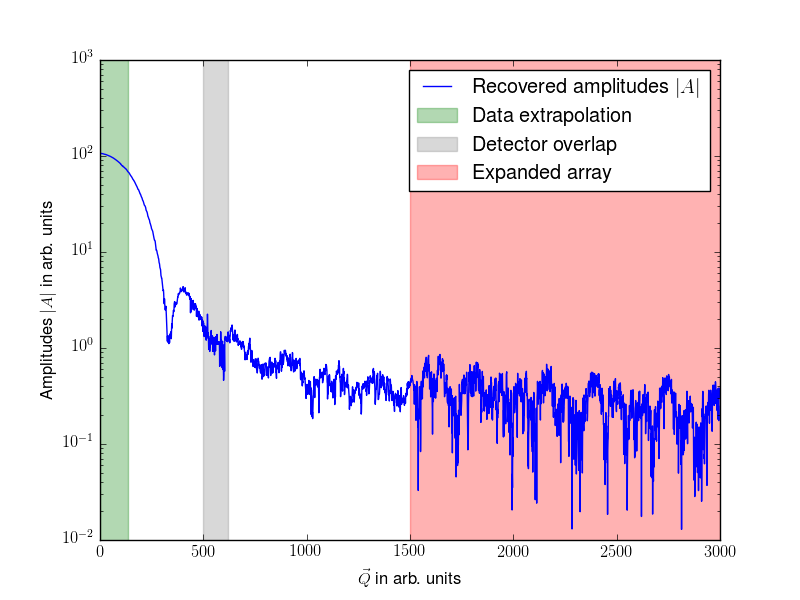
\includegraphics[width=0.49\textwidth]{images/results/amplitude-discussion.png}
		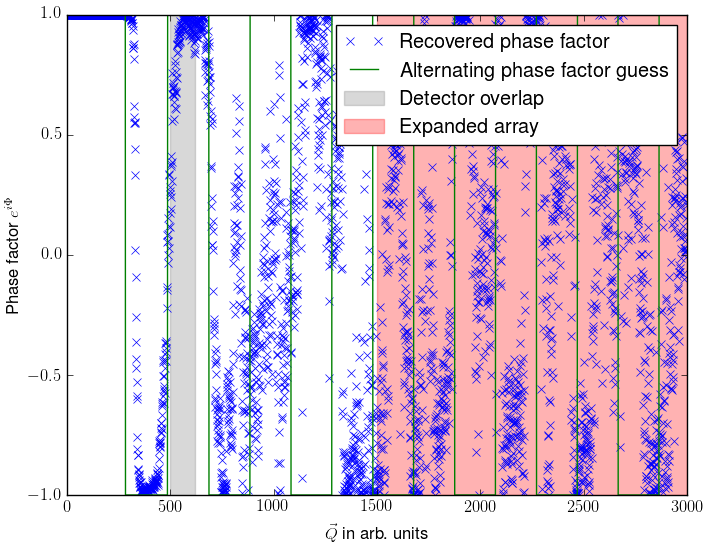
\includegraphics[width=0.49\textwidth]{images/results/phase-discussion.png}
	\caption{Recovered amplitudes $\left|A\right|$ and phase factor of the 1D phase retrieval (see section \ref{sec:1d-proj-and-phase-reconstruction}). The green and red background indicates the space where initial data points were extrapolated. The gray area discloses the detector overlap.}
	\label{fig:amplitude-phase}
\end{figure}
For the sake of completeness, the recovered modulo of the amplitude $\left|A\right|$ and the recovered phase factor are shown in figure \ref{fig:amplitude-phase} for the data points at $\Delta t =800$ fs. The measured amplitudes $\left|A\right|$ have been replaced in the space with white background. The initial data in with the green background was interpolated using the anticipated scattering of a sphere. The grayed area is from the pnCCD detector overlap and the red background are extrapolated data points from the scattering of a sphere. The red area therefore increases the resolution. The data points of the k-times iterated Fourier-space function $G'_{k}(\vec{Q})$ in the white area were replaced with the original data set while $G_{k}(\vec{Q})$ was allowed to evolve freely in the remaining area. The phase factor retrieval starts with an initial guess of alternating signs per diffraction ring of the sphere and then evolves freely. One can see how the recovered phase factor is alternating as one would expect from the scattering of a sphere.\\
% 2D RECONSTRUCTIONS
\begin{figure}
	\centering
		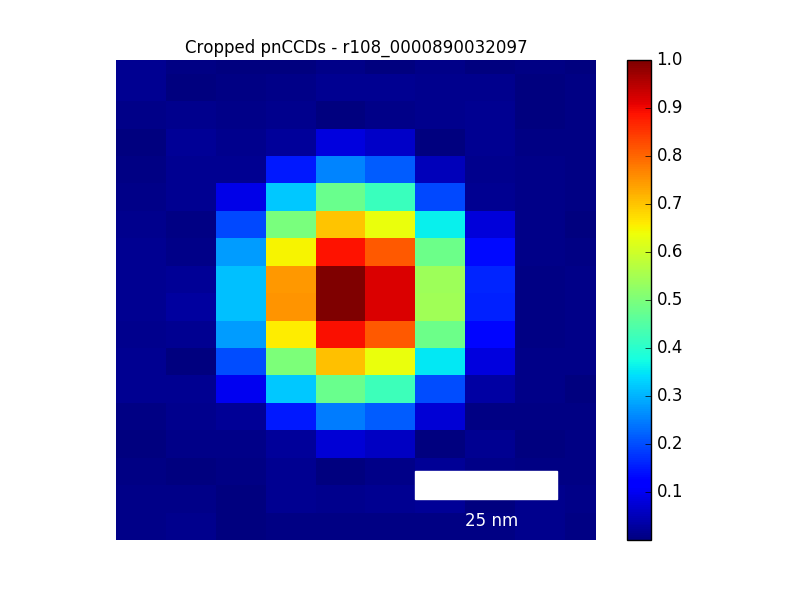
\includegraphics[width=0.49\textwidth]{images/results/Xe_0_fs.png}
		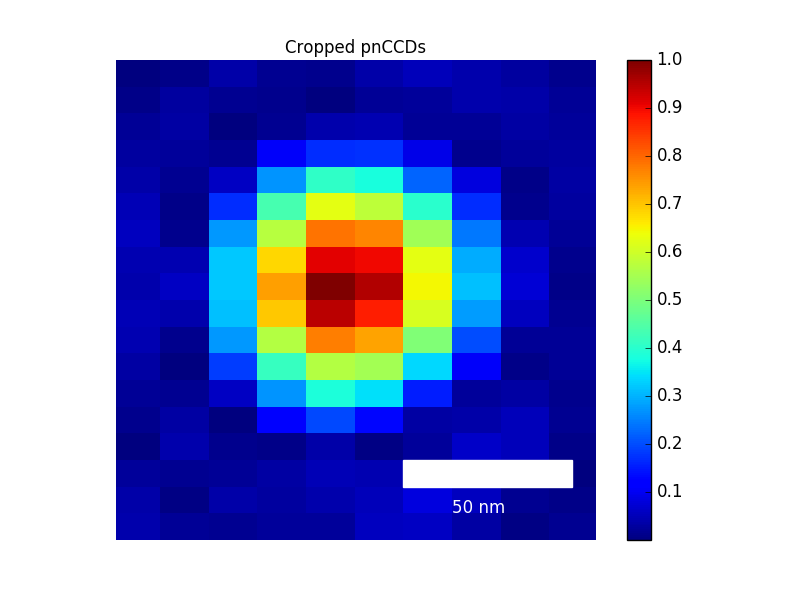
\includegraphics[width=0.49\textwidth]{images/results/Xe_800_fs.png}
	\caption{Single-shot 2D reconstructions of diffraction pattern from single Xe-cluster. The left image shows a $\sim 50$ nm radius Xe-cluster at a pump--probe delay $\Delta t=0$ fs. The cluster has a spherical or arguably icosahedron electron distribution that is distinct compared to the background. The right image shows a $\sim 50$ nm radius Xe-cluster at a time delay $\Delta t=800$ fs that shows a similar symmetry but due to the loss of scatterer (see fig \ref{fig:number-of-scatterer}), the signal to noise ratio decreases and a ringing that is likely from the support structure in the phase-retrieval process is surrounding the cluster.}
	\label{fig:Xe-2D-reconstructions}
\end{figure}
Figure \ref{fig:Xe-2D-reconstructions} shows 2D reconstructions of single Xe-cluster at $\Delta t = 0$ fs (left) and $\Delta t=800$ fs (right). The cluster appear generally spherical, however an icosahedral shape is imaginable. Both cluster have a radius of $r\approx 50$ nm. The reconstructions constitute one of the smallest objects recovered with CDI at the time of writing. The minimal resolvable feature size in these images is $\sim 14\times \sim 6$ nm along the $X\times Y$-axis (see section \ref{sec:resolution-discussion}). The reconstruction at $\Delta t=800$ fs shows a ringing around the actual cluster, which is likely an artifact of the spherical support structure. This ringing becomes visible due to the lower signal-to-noise ratio compared to the reconstruction at $\Delta t=0$ fs. The lower signal is due to the in figure \ref{fig:number-of-scatterer} described loss of electrons.
%
%
%
\section{Time-resolved response of highly ionized Xe-atoms in intense X-ray pulses}
%%%%%%%%%%%%%%%%%%%%%%%%%%%%%%%%%%%%%%%%%
%- Xe iToF dynamics\\
%- Slightly more of Xe higher charge-states present at longer delays.
%%%%%%%%%%%%%%%%%%%%%%%%%%%%%%%%%%%%%%%%%
\begin{figure}
	\centering
		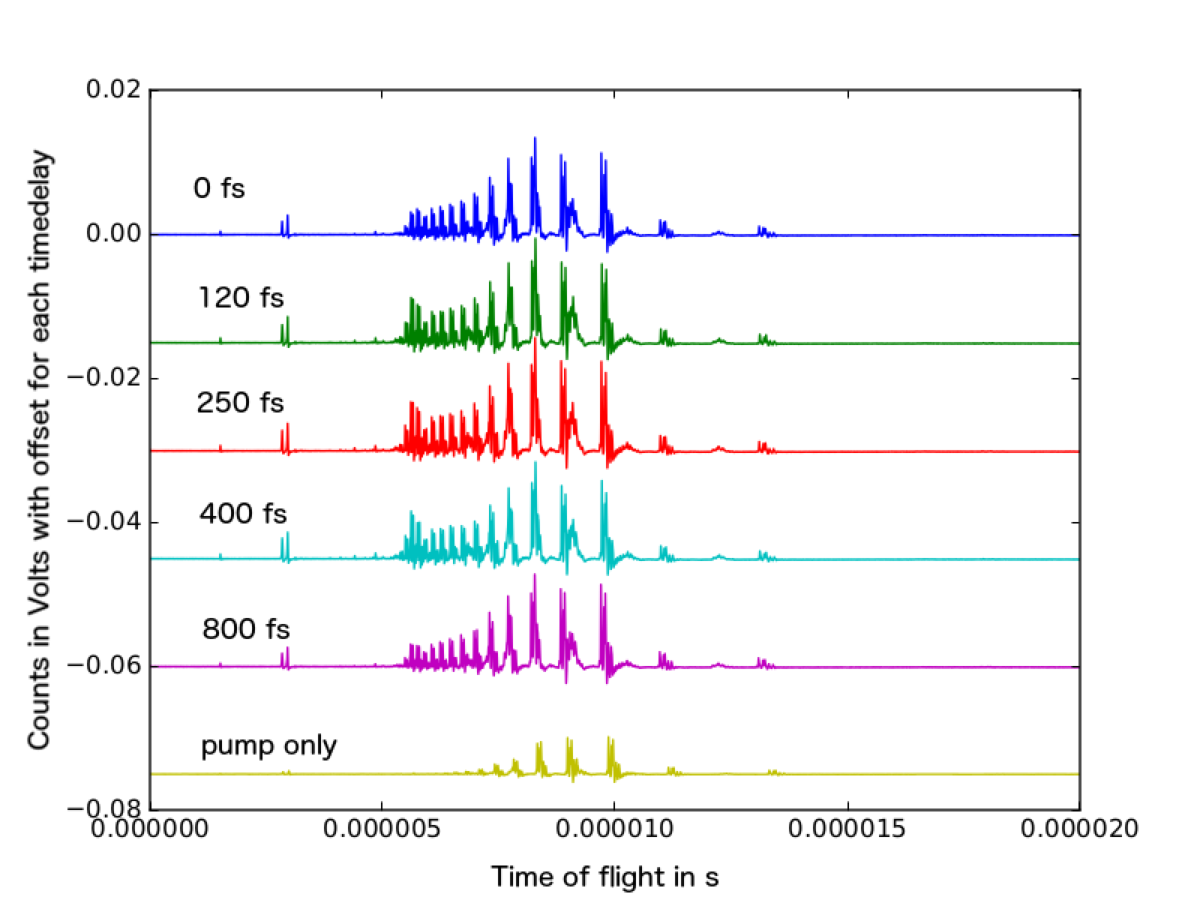
\includegraphics[width=0.49\textwidth]{images/results/TOF-atomic-xenon.png}
		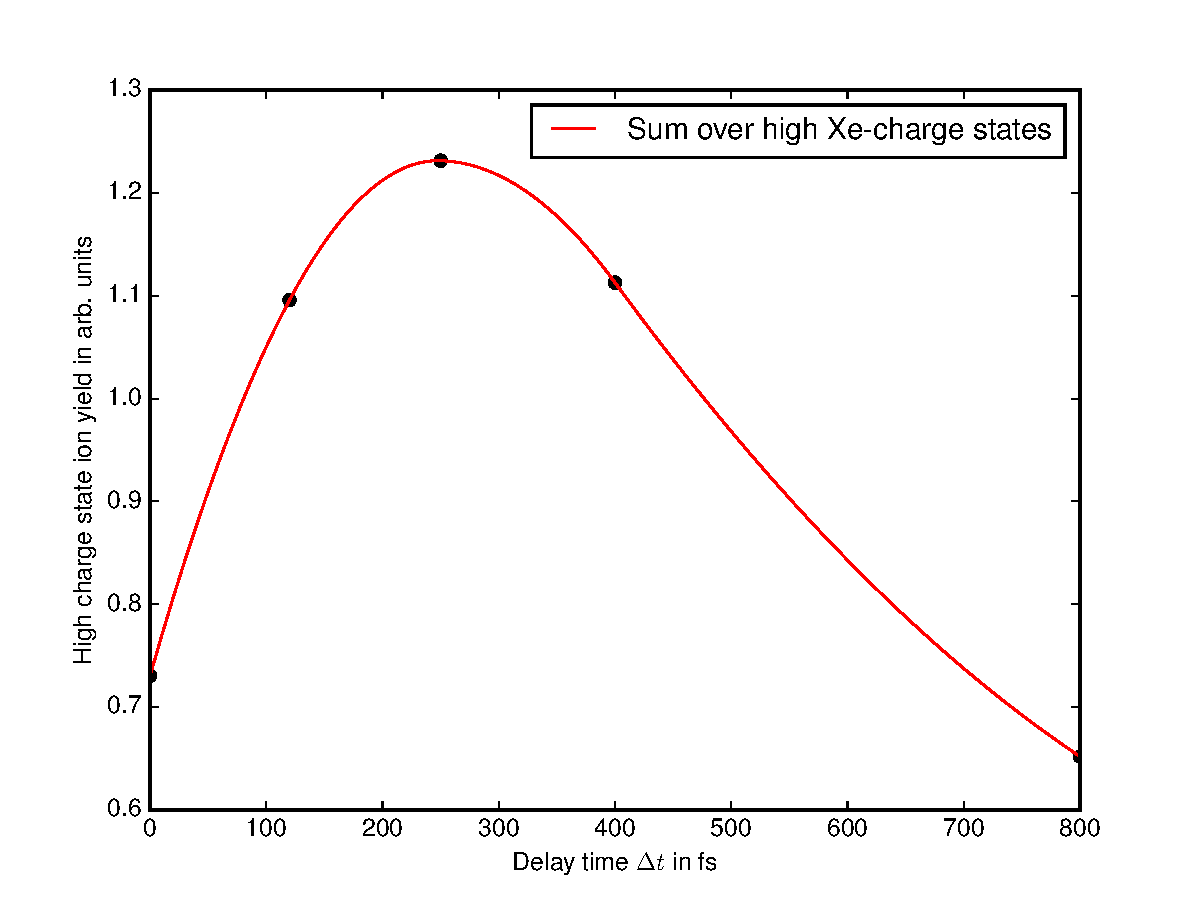
\includegraphics[width=0.49\textwidth]{images/results/atomic-charge-state-time-resolved.pdf}
	\caption{Atomic xenon ion time-of-flight data shows resonant type behavior. As the X-ray pump-pulse traverses through the xenon ions, the 3d-subshell becomes highly ionized and thus the atom increasingly transparent for the probe-pulse ($\Delta t \approx 0-120$ fs). The electron-holes have a longer lifetime due to the highly ionized subshell. After the Auger decay populates the 3d-subshell, the atom becomes less transparent and the X-ray pump-pulse efficiently ionizes the atoms ($\Delta t \approx 250$ fs). Eventually other relaxation processes, e.g. fluorescence, dissipate energy from the pump-pulse away from the nanosample leading to a lower high charge states.}
	\label{fig:TOF-atomic-xenon}
\end{figure}
Ion time of flight traces of atomic xenon at different time delays $\Delta t = \{0, 120, 250, 400, 800\}$ fs and X-ray pump only data is shown in figure \ref{fig:TOF-atomic-xenon}. The time of flight data show a resonance type of behavior of the atomic xenon high charge states with a peak of high-charge state yield at $\Delta t = 250$ fs. The initial increase of high xenon charge states can be explained with intensity-induced X-ray transparency \citep{Young-2010-Nature}. In the present study, the xenon 3d-subshell is efficiently ionized by the X-ray pump pulse. These electron-holes are typically repopulated on the few femtosecond timescale due to the Auger decay, however, the increasingly ionized atom has longer electron-hole lifetimes. It has been measured that $\text{Ne}^{8+}$ has core-hole lifetimes of $~230$ fs. But why does the charge state distribution then not level out for later delays $\Delta t > 250$ fs? When the strongly pumped atom does not absorb energy near saturation, slower relaxation processes, for example fluorescence, occur that effectively dissipate energy from the nanosample, thereby reducing the average ionization level.\\
%\begin{figure}
	%\centering
		%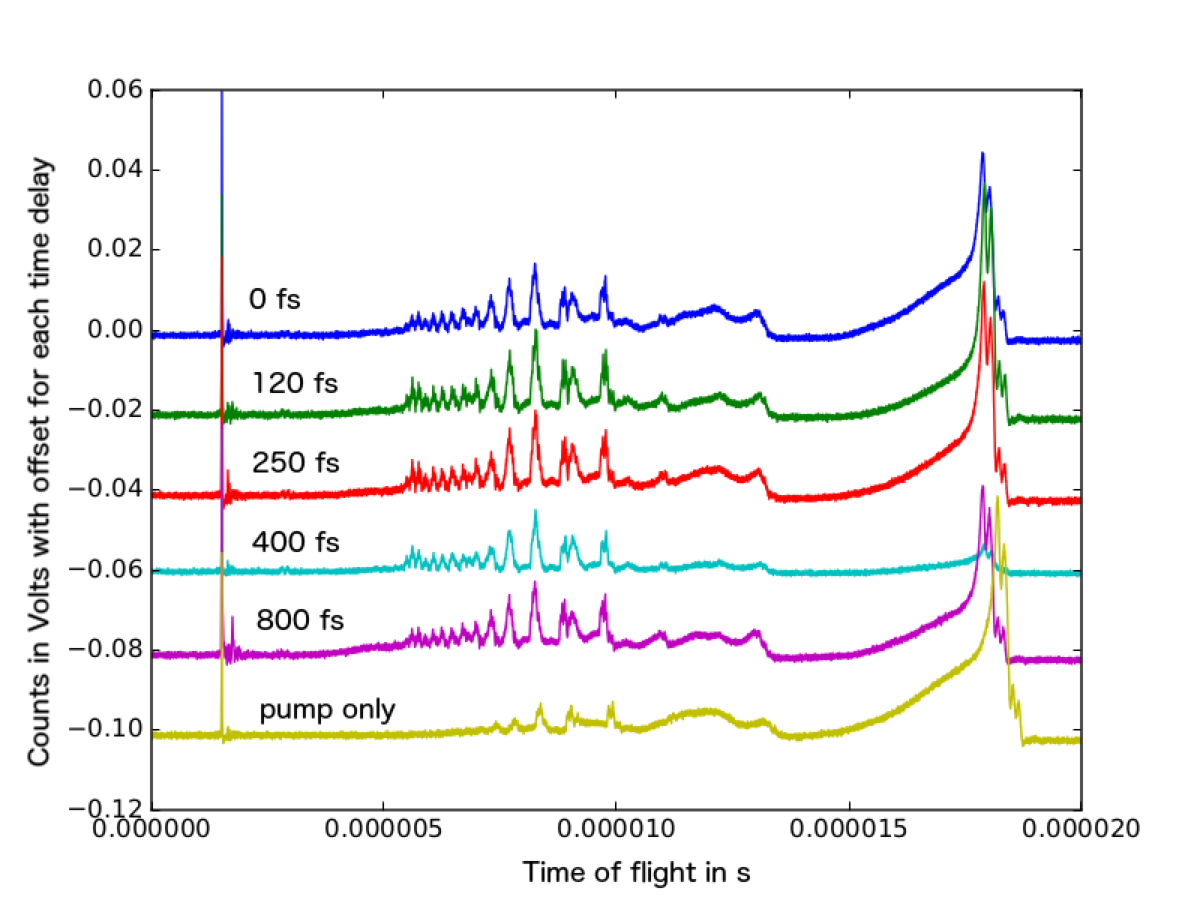
\includegraphics[width=0.80\textwidth]{images/results/TOF-small-cluster-xenon.png}
	%\caption{caption}
	%\label{fig:TOF-small-cluster-xenon}
%\end{figure}
%Figure \ref{fig:TOF-small-cluster-xenon} shows ion time of flight traces of small xenon cluster cluster at different time delays $\Delta t = \{0,120,250,400,800\}$ fs and X-ray pump only data. To create xenon cluster on the order of XXX nm radius the reservoir pressure in the source has been changed to $p_{0}=6$ bar. The data show similar resonant behavior as in the atomic case. Xenon high-charge states peak at a X-ray pump -- X-ray probe delay of 250 fs and start decrease at higher delays. At longer time of flight durations of 10 $\mu$s and beyond the small cluster signal dominates. Due to the short run times, the fluctuations of the cluster source vary the cluster signal significant.\\
%\begin{figure}
	%\centering
		%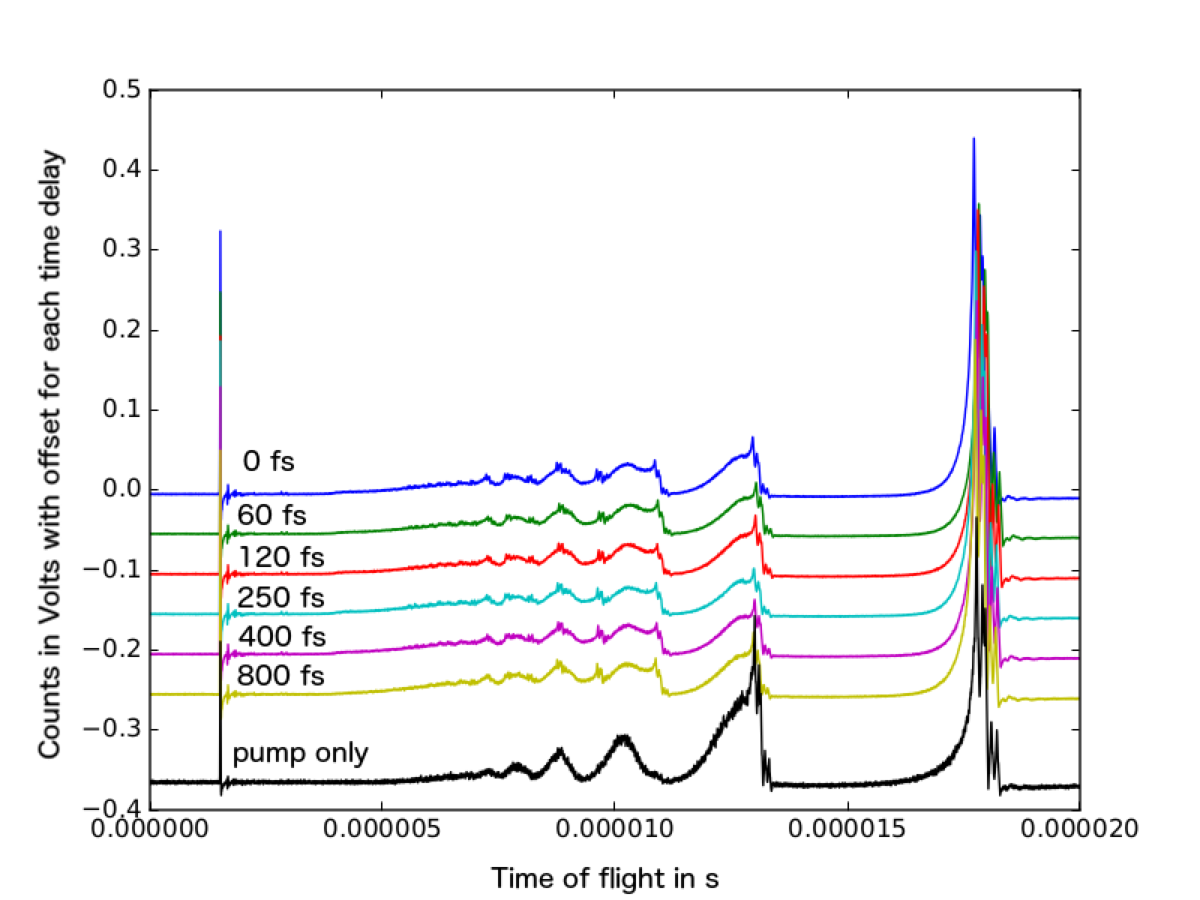
\includegraphics[width=0.80\textwidth]{images/results/TOF-regular-cluster-xenon.png}
	%\caption{caption}
	%\label{fig:TOF-regular-cluster-xenon}
%\end{figure}
%Ion time of flight traces of larger clusters can be found in figure \ref{fig:TOF-regular-cluster-xenon}. Here a mean Xe-cluster radius of $\sim 61$ nm is observed. The time delay between X-ray pump and X-ray probe has been set to $\Delta t=\{0,60,120,250,400,800\}$ and also the pump only data is shown. The data show that the cluster type of signal is dominating the trace. At a time delay $\Delta t=800$ fs, the xenon high-charge states increase, while no other dynamic appears obvious from the average data. The larger cluster ensemble may undergo a similar resonant type behavior as atomic xenon, however, the large cluster ensemble seem to affect the ionization pathways and thus the timescale of the resonant type behavior.\\
%Summarizing, atomic xenon, xenon cluster of mean radius $\sim XXX$ nm and Xe-cluster of average radius $\sim 61$ nm were investigated using a X-ray pump -- X-ray probe setup coincidently measuring spectroscopy and coherent diffractive imaging data. The ion spectroscopy data of atomic xenon high charge states show a resonant type behavior as the time delay $\Delta t$ is varied from 0 fs to 800 fs. The effect peaks, i.e. is resonant around 250 fs. Small xenon cluster exhibit a similar behavior as atomic signal because atomic signal is dominating the high-charge states. The signal from larger xenon cluster of radii $\sim 61$ nm is dominated by xenon charge fragments. An increase in the xenon high-charge states is observed at 800 fs, allowing us to conclude that the ionization dynamics have changed. It is interesting to note that altough larger cluster absorb overall more energy, the ensemble of atoms that is bound in the cluster is able to collectively change, here slow, ionization pathways. This behavior may be reproduced in other nano-samples such as bio-molecules or artifical tamper layers.
%
%
%
%%%%%%%%%%%%%%%%%%%%%%%%%%%%%%%%%%%%%%%%
\section{Time-resolved response of highly ionized He-cluster and with xenon doped He-cluster}
%%%%%%%%%%%%%%%%%%%%%%%%%%%%%
% - Subsection for iToF data, important to compare to HeXe data.
%%%%%%%%%%%%%%%%%%%%%%%%%%%%%
\begin{figure}
	\centering
		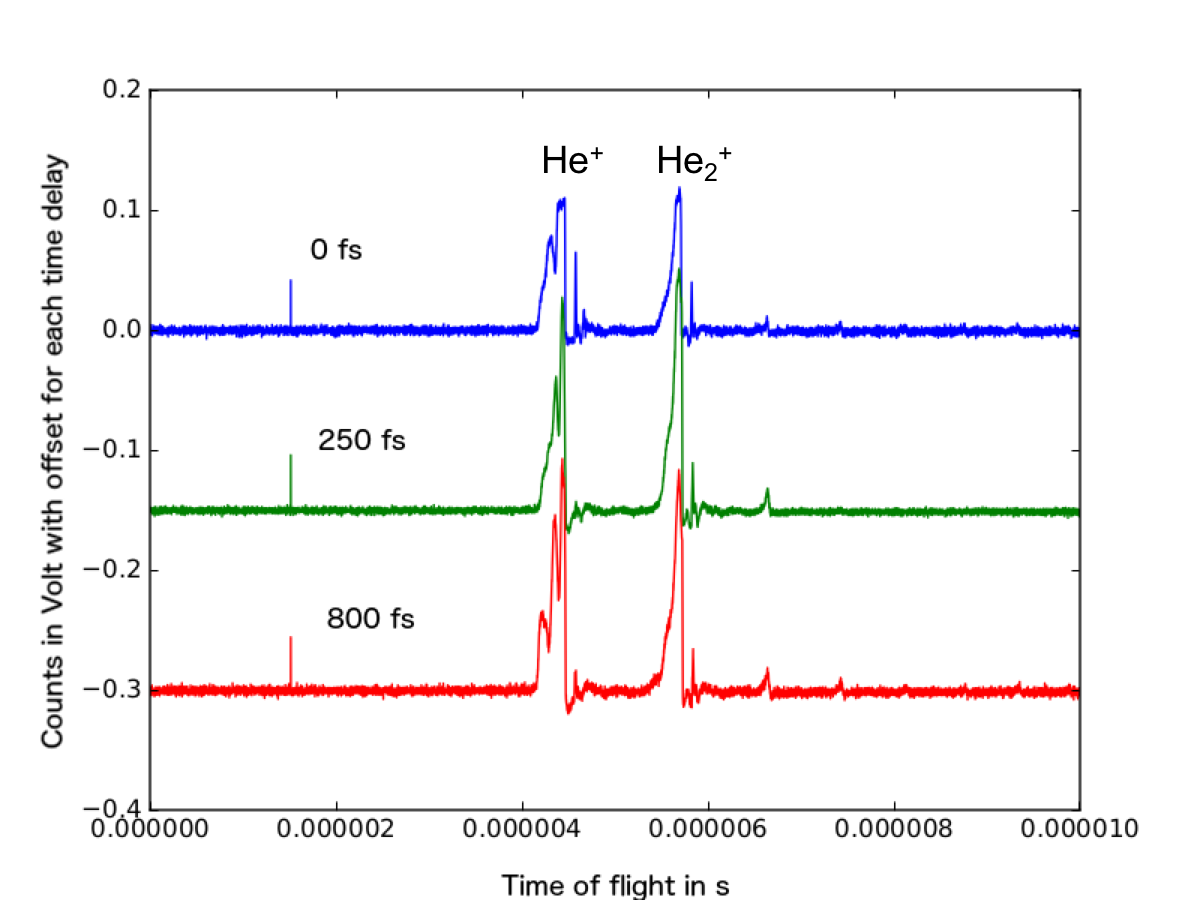
\includegraphics[width=0.65\textwidth]{images/results/TOF-helium-cluster.png}
	\caption{Ion time of flight traces of He-cluster with a radius of $r_{\text{He}}\approx 810$ nm. Although minor changes in the charge fragmentation are observed, we shall note that there are no $He^{2+}$ ions in this data. The absorption cross-section of helium are too low to lead to doubly charged states \citep{Ho-2016-PC}.}
	\label{fig:TOF-helium-cluster}
\end{figure}
The response of clusters in highly intense X-ray radiation is more complex than the atomic signal. Size dependent effects \citep{Schorb-2012-PRL,Schutte-2015-JPhysB} and recombination effects in the nanoplasma \citep{Schutte-2014-PRL} alter the sample's ionization pathways. Figure \ref{fig:TOF-helium-cluster} shows ion time of flight data of pristine He-cluster charge fragments at pump--probe delays $\Delta t=\{0, 250, 800\}$ fs. The pristine He-droplets have a radius of $r_{\text{He}}\approx 810$ nm or $\left\langle N_{\text{He}}\right\rangle\approx 5\cdot 10^{10}$ on average using the relation \citep{Gomez-2011-JCP}
\begin{equation}
r_{\text{He}}=0.22 (N_{\text{He}})^{\frac{1}{3}}\ [\text{nm}].
\end{equation}
The data show overall a similar behavior regardless of the delay $\Delta t$, although minor changes in the charge fragmentation distribution can be made out. More importantly for the reference purposes, the traces indicate no contribution of doubly charged helium atoms. The lack of double charged helium can be explained to the comparably low absorption cross-sections of helium (see table \ref{tab:helium-xenon-ionization}) \citep{Ho-2016-PC}.\\
\begin{figure}
	\centering
		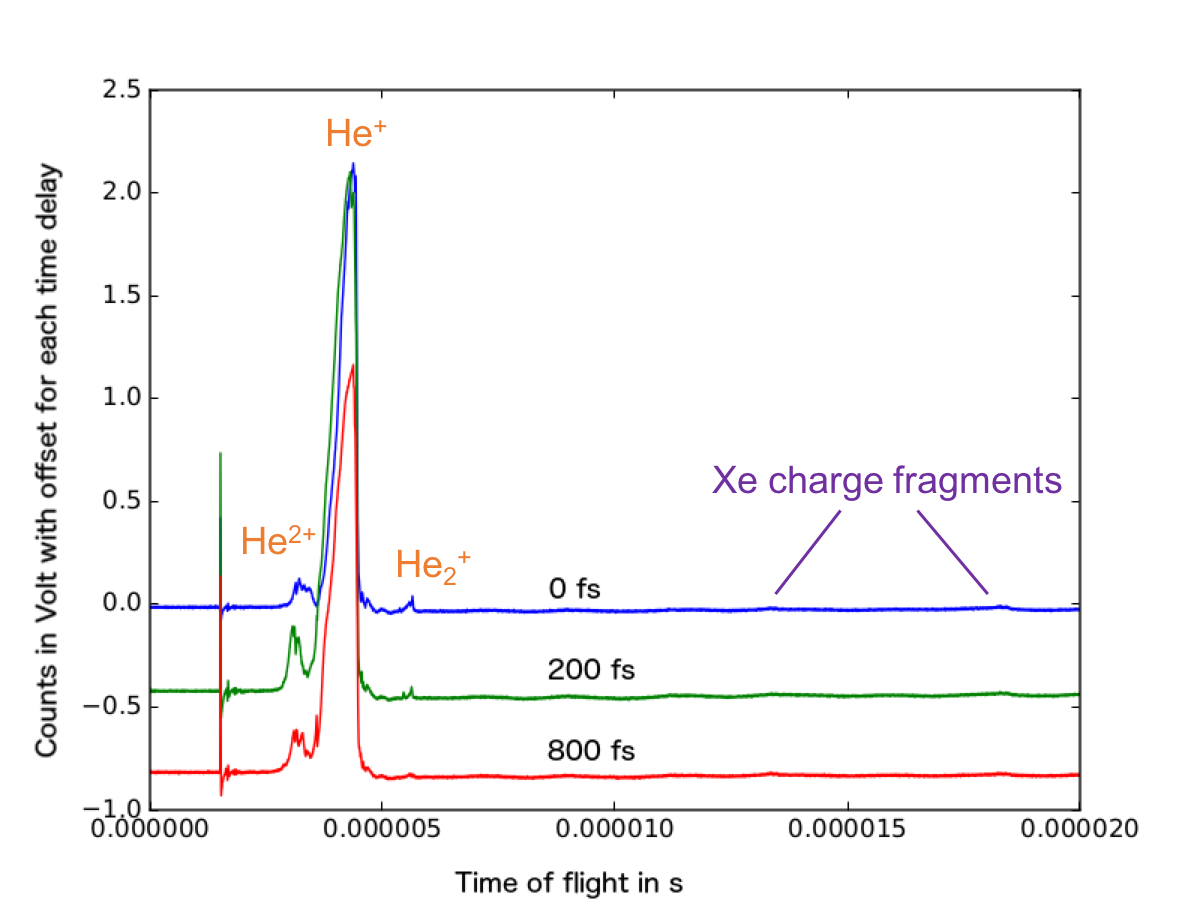
\includegraphics[width=0.65\textwidth]{images/results/TOF-helium-xenon-cluster-60.png}
	\caption{Ion time of flight spectra of He-cluster with $\left\langle N_{\text{He}}\right\rangle\approx 2\cdot 10^{10}$ particles and $\sim 0.6\%$ as many xenon particles. The Xe-atoms absorb X-rays efficiently and transfer the absorbed energy to the He-atoms. The Xe-ions recombine and only few xenon charge fragments are observed. Due to the energy transfer, doubly charged He-ions are detected and the KER is increased as well. As the delay time $\Delta t=\left\{0,200,800\right\}$ is varied, the system undergoes a resonant type behavior that is attributed to the ionization dynamics of Xe-atoms. More in text.}
	\label{fig:TOF-helium-xenon-cluster-60}
\end{figure}
Strongly with xenon doped helium cluster time of flight traces are shown in figure \ref{fig:TOF-helium-xenon-cluster-60}. Here the He-droplets have a radius of $r\approx 600$ nm or $\left\langle N_{\text{He}}\right\rangle\approx 2\cdot 10^{10}$ particles with a $\sim 0.6\%$ doping level of xenon. So here, the helium depletion is $\sim 62\%$ (see section \ref{sec:heterogeneous-cluster}). Most notably on the one hand is the presence of $\text{He}^{2+}$ ions and a strongly increased signal from $\text{He}^{+}$ ions. And on the other hand, only few xenon charge fragments are observed. This is counter intuitive as the absorption cross-section from xenon is vastly higher than from helium (see table \ref{tab:helium-xenon-ionization}). We can therefore synthesize that, one, there must be an efficient, ultrafast energy transfer process from the xenon particles to the He-droplet, and two, that the helium atoms function as electron reservoir as the initially photoionized xenon atoms are hardly detected. As the time delay $\Delta t$ is varied, we observe that the He-ion signal shows a resonant type behavior. At $\Delta t = 200$ fs, the signal from $\text{He}^{2+}$ and $\text{He}^{+}$ peaks, however, the helium signal is less intense at the delay times $\Delta t = 0$ and 800 fs. We can make use of the earlier discussion from figure \ref{fig:TOF-helium-cluster} and \ref{fig:TOF-atomic-xenon} and conclude that this behavior does not originate from the absorption and ionization dynamics of the He-cluster but rather of the xenon atoms that the He-droplet has been doped with.\\
%Comparing the data from figure \ref{fig:TOF-helium-cluster} and \ref{fig:TOF-helium-xenon-cluster-60} allows us to conclude that xenon cluster transfer energy to the helium cluster that they are embedded in. This process is very efficient since the resonant behavior that origins from the xenon atoms is constituted in the helium signal, while the xenon signal steadily decreases. Therefore,  This behavior is similar to \citep{Hoener-2008-JPB} but differs in it's geometric arrangement.\\
\begin{figure}
 	\centering
 		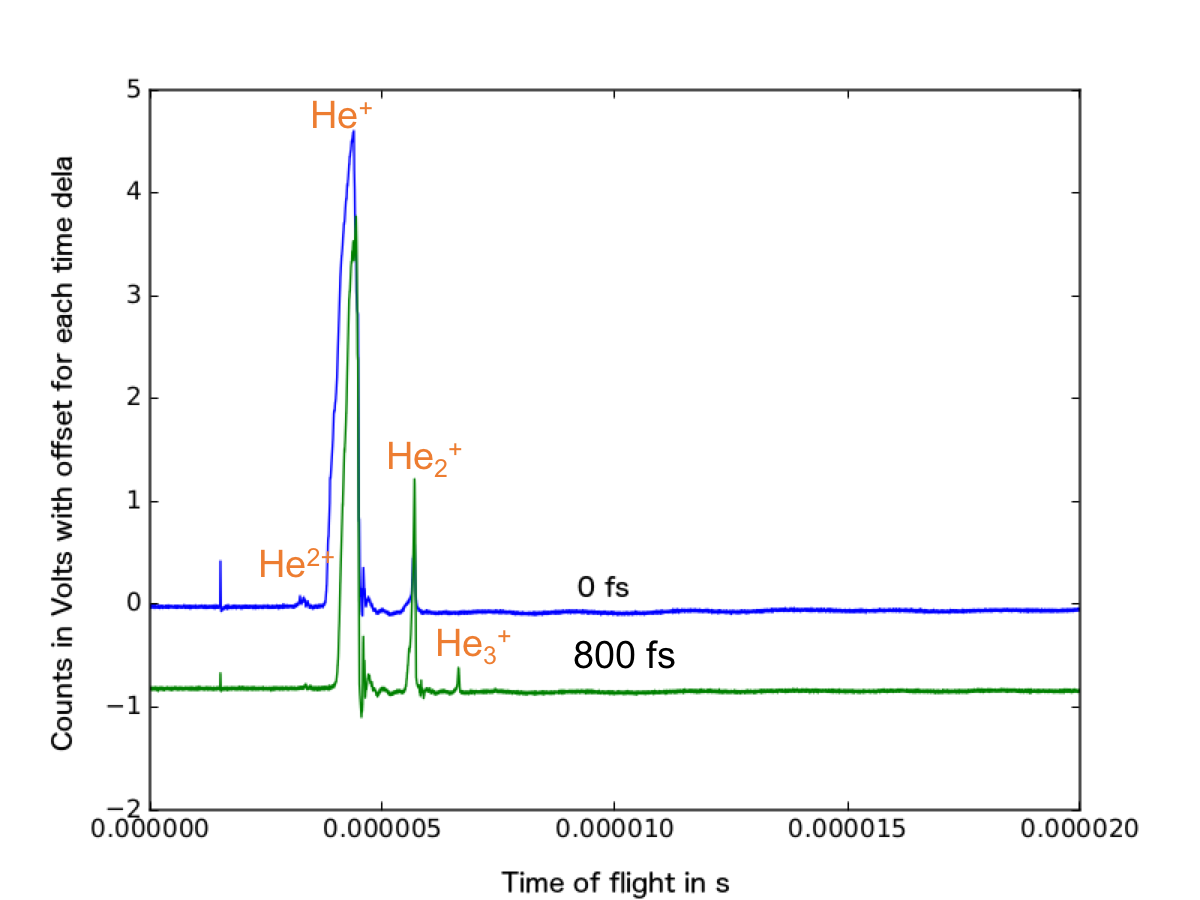
\includegraphics[width=0.65\textwidth]{images/results/TOF-helium-xenon-cluster-13.png}
 	\caption{Ion time of flight spectra of He-cluster with $\left\langle N_{\text{He}}\right\rangle\approx 4.4\cdot 10^{10}$ particles and $\sim 0.06\%$ as many xenon particles. These lesser doped He-cluster show a lower He-ion count due to the reduced absorption of the Xe-atoms. As the delay time $\Delta t=\left\{0,800\right\}$ is varied, the system shows dynamics in the population of the ion-states and it is likely  that these dynamics are also to be attributed to the atomic xenon ionization dynamics. More in text.}
 	\label{fig:TOF-helium-xenon-cluster-13}
\end{figure}
Figure \ref{fig:TOF-helium-xenon-cluster-13} shows ion time-of-flight data of with $r\approx 775$ nm radius He-droplets and a $0.06 \%$ level doping at pump--probe delays $\Delta t=\{0, 800\}$ fs. So here, the helium depletion is measured to be $\sim 13\%$. We note, again, the presence of $\text{He}^{2+}$ ions and more signal from $\text{He}^{+}$ ions. However, the compared to the stronger doped data these peaks are less intense. Qualitatively this can be explained with the less strong doping, because the X-ray absorption from the xenon atoms and subsequent energy transfer to the helium atoms dominate the helium ion characteristics. Less doping results in fewer photon absorption processes and thus less energetic helium ion characteristics. At different time delays $\Delta t$, the height of each peak shifts. The $\text{He}^{2+}$ and $\text{He}^{+}$ states become less frequent but a stark increase in $\text{He}_{2}^{+}$ and $\text{He}_{3}^{+}$ ion peaks is observed. It is likely that the ionization dynamics undergo a resonant type behavior, however, there are too few data points to investigate this in detail.\\
Summarizing, pristine He-droplets show little dynamics as the time delay $\Delta t$ is varied and only singly charged $\text{He}^{+}$ ions are measured. If the He-droplets are doped with xenon, a doubly charged $\text{He}^{2+}$ ions are detected, the kinetic energy release (KER) is stronger and the time-of-flight data reveals dynamics that are comparable to atomic xenon, when the delay $\Delta t$ is varied. As the xenon doping is increased, the presence of $\text{He}^{+}$ and $\text{He}^{2+}$ ions after the pump--probe is more frequent. This data suggests an ultrafast and efficient energy transfer from the xenon atoms to the helium atoms, for example through collisions. The helium particles furthermore act as an electron reservoir such initially photoionized xenon atoms recombine and only few xenon charge fragments are detected by the time of flight spectrometer. The underlying idea that a low-Z material acts as a electron supplier for the high-Z material has also been studied similarly in \citep{Hoener-2008-JPB}.
%
%
%
\section{Heterogeneous helium-xenon cluster core-shell system}\label{sec:helium-data}
%%%%%%%%%%%%%%%%%%%%
% - Presentation of He data
%%%%%%%%%%%%%%%%%%%%%%%%%%
It is not well known how heterogeneous helium-xenon cluster form a core-shell system. As described in section \ref{sec:heterogeneous-cluster}, the liquid helium cluster picks up xenon atoms as it traverses the doping unit. The xenon atoms move unhindered in the superfluid helium and eventually the xenon atoms condense to energetically favorable cluster structures. \citep{Gomez-2014-Science} reports that at a doping level of $0.02\%$, i.e. 5000 more helium atoms than xenon atoms, multiple smaller clusters form and locate at vortexes of the rotating helium droplet. However, it is unknown how xenon atoms arrange in non-rotating droplets and also at higher doping levels. The two competing hypotheses are, one, xenon atoms condense to one large cluster within a helium droplet, two, multiple smaller Xe-cluster form within a droplet. Let us call hypothesis two a plum-pudding core-shell system \textit{plum pudding core-shell system}\footnote{The name plum-pudding model comes from J.J. Thomson's model of the atom in 1904 and has here been reused to describe the arrangement of atoms in heterogeneous (rare-gas) clusters.} that we can further divide into a few (larger) and many (smaller) scatterer scenario.\\
\begin{figure}
 	\centering
 		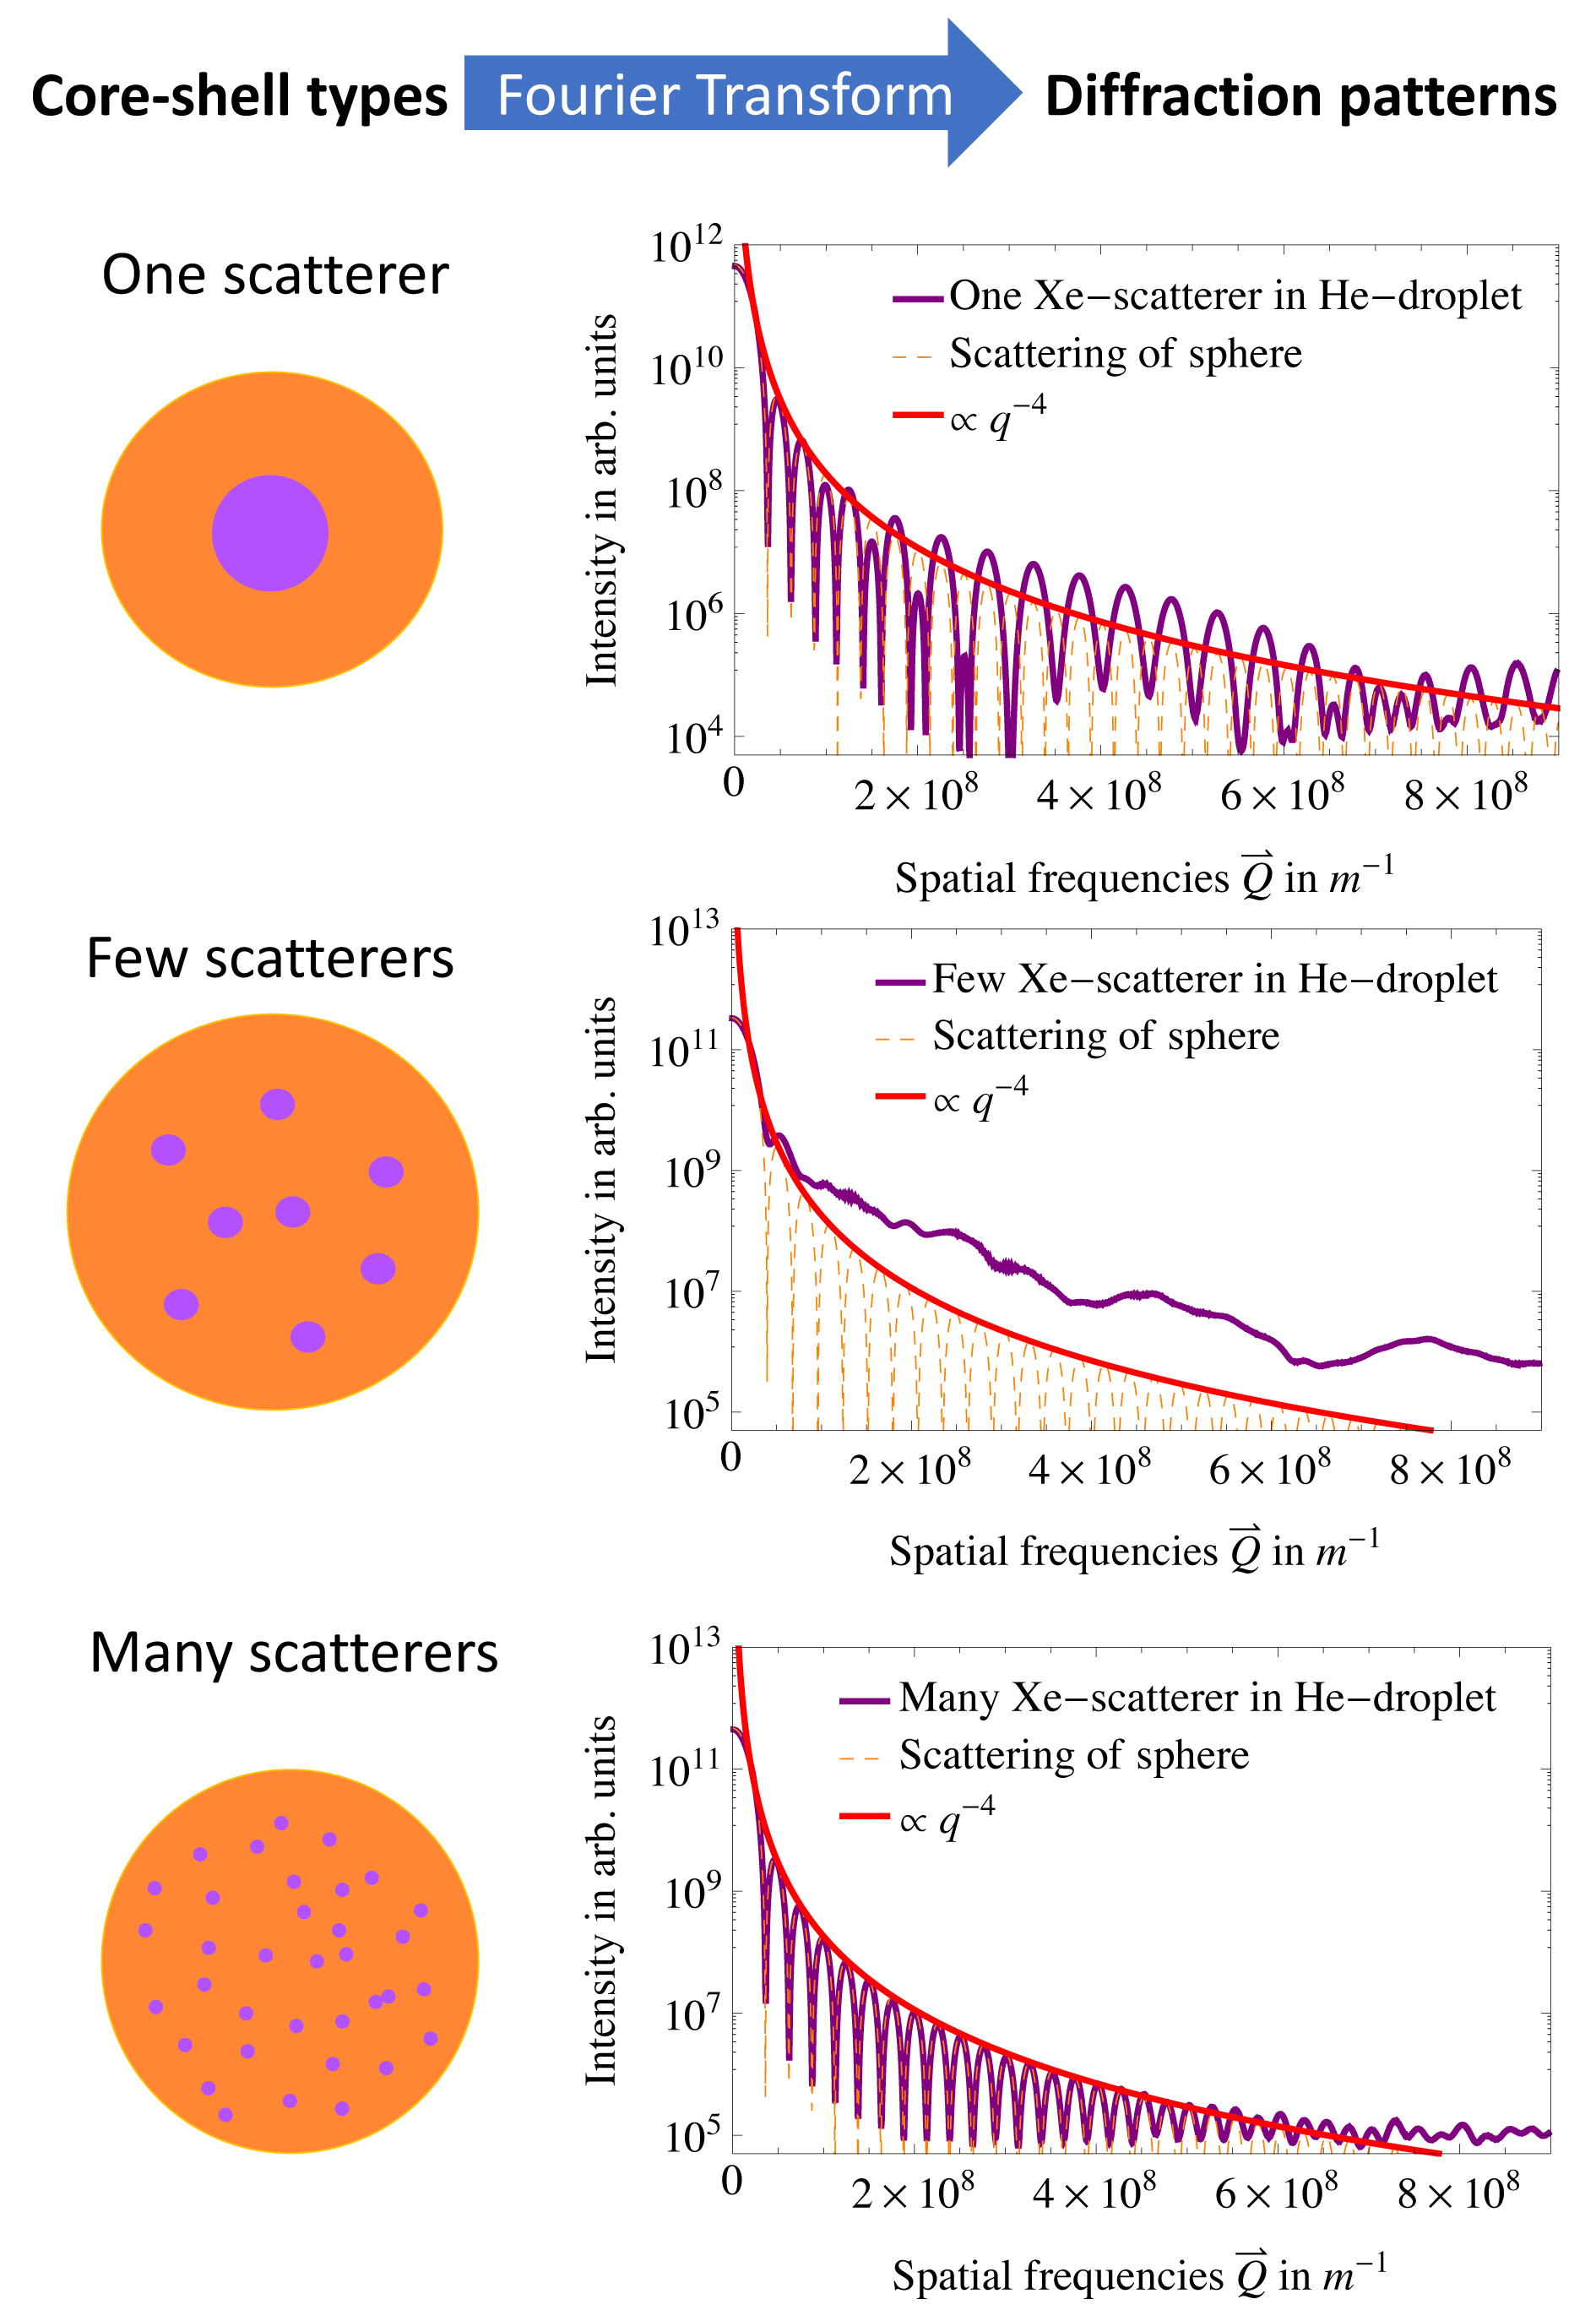
\includegraphics[width=0.80\textwidth]{images/results/plum-pudding.png}
 	\caption{Potential arrangement of xenon atoms in a liquid helium cluster and corresponding 1D diffraction patterns. The He-droplet has a radius of $\sim 125$ nm and the Xe-doping level is at $\sim 20\%$. The extreme cases, i.e. one xenon scattering center $N_{\text{sc}}=1$, few scatterer $N_{\text{sc}}=8$ and many scatterer $N_{\text{sc}}=100$ are shown to illustrate their impact on diffraction pattern. In short, the scattering pattern is dominated by the signal from the He-droplet at low $\vec{Q}$-values and at large $\vec{Q}$-values the signal is dominate by the $Xe-clusters$. This is mostly due to the size of the Xe-clusters and smaller scattering centers are resolved at larger scattering angles. More in text.}
 	\label{fig:HeXe-plum-pudding}
\end{figure}
The core-shell arrangements are shown in figure \ref{fig:HeXe-plum-pudding} along with their Fourier-space representations. The shown He-droplet has a radius of $r\approx 125$ nm and a constant xenon doping level of $\sim 20\%$, i.e. the figure shows an artistic representation of the simulated real-space core shell systems. These 2D-simulations are described in more detail in section \ref{sec:2d-simulations}. In the illustration, it becomes obvious that the formation of the xenon atoms within the He-droplet dominates the scattering pattern, which is due to the Xe-cluster density being $\sim 25.8$ times larger than the density of liquid He-droplets. In simplified terms, the one scatterer case shows a large modulation in the diffraction image, which comes from the Xe-core and a small, more intense modulation that comes from the He-shell (similar to orange, dashed line). At low spatial frequencies $\vec{Q}$, the He-droplet dominates the signal on the diffraction image and at large spatial frequencies $\vec{Q}$, the Xe-cluster influence is more concise. Ultimately, this is related to the size of each cluster and the mentioned modulations in Fourier-space. In the few scatterer case with $N_{\text{sc}}=8$ scattering centers, the diffraction pattern at low spatial frequencies $\vec{Q}$ is still dominated from the He-shell and at large spatial frequencies $\vec{Q}$ from the Xe-cores. However, the diffraction image appears more complex structured at large $\vec{Q}$-values due to intense decentered scatterers. Also, the average scattering intensity is well above the scattering of a sphere (red line) that has been fitted onto the zeroth diffraction order. The location of the few scatter plays a lesser role in the 1D projection of the 2D diffraction image, as long as the scattering centers are distributed throughout the He-droplet, i.e. do not reproduce the case of one scatterer. Finally, the many scatterer case with $N_{\text{sc}}=100$. The 100 within the He-droplet randomly distributed scatterer are significantly reduced in size to match the constant xenon doping level of $\sim 20 \%$. For the outer shape, the small clusters appear similar to constant electron density increase, which is visible at low to mid $\vec{Q}$-values thus the scattering is practically identical to the scattering of a similar sized sphere (orange, dashed line). Only at large $\vec{Q}$-values that reveal small structures, the Xe-scatterer start to dominate the signal, i.e. signal is above the envelope function of the scattering of the sphere.\\
To quantify the effect of the Xe-cluster size using a crude estimate. For that we can make use of Abbe's criterion \eqref{eq:abbe-criterion} and the wave vector definition \eqref{eq:Q-scattering-angle} to write down the minimal resolvable feature size $d$ as follows
\begin{equation}
d = \frac{2\pi}{\left|\vec{Q_{r}}\right|},
\label{eq:diameter-estimate}
\end{equation}
with $\left|\vec{Q_{r}}\right|$ being the point in reciprocal space, where the signal starts to be dominated by the smaller structures, here the Xe-clusters. To move ahead, we can relate the resolvable feature size $d$ to the radius $r$ of the smaller spherical structures via $d\approx 2 r$. This relation works well for the one-scatterer case $r\approx 15$ nm. However, as the structures become more complex one has more spatial frequency contributions from not only the smaller structures, i.e. the Xe-cluster, but also the space in between smaller structures and the space from the smaller structures to the boundary of the system, i.e. the He-droplet. Multiple smaller structures thus form a \textit{superstructure}\index{superstructure} that appears larger than its individual components when estimated via equation \eqref{eq:diameter-estimate}. For the plum-pudding cases the Xe-cluster form superstructures with the He-droplet. This superstructure is $\sim 3$ times larger in the few scatterer case and $\sim 10$ times larger in the many scatterer case than its individual, simulated Xe-cluster components.\\
%The study of diffraction patterns thus gives insight into the heterogeneous core-shell system. Ultimately, the structure of a heterogeneous HeXe-cluster must be understood to further conclude about effects of radiation damage. To study the diffraction pattern of heterogeneous cluster 2D simulations were developed that simulate the electron density of a cluster and then Fourier transform these into Fourier-space. The 2D diffraction images are then projected onto 1D to be compared efficiently. More details about this method can be found in section \ref{sec:2d-simulations}.\\
%The 2D electron density simulations show that Xe atoms arrange as few randomly orientated clusters within the He-droplet. The data in figure \ref{fig:HeXe-cluster-60} shows several cases of Xe arrangement within the He-droplet. First, looking at the extreme cases of no Xe-scatterer (n=0) and many small Xe-scatterer $(n=100)$ show vastly different scattering pattern than measured. Only the case of few Xe-scatterer $(n\approx 10)$ reproduces the in the experiment measured data. This approach also allows a precise determination of the Xe-doping level on a shot-to-shot basis as the size of the Xe-cluster within the He-droplet can be adapted to fit the measurement. The overall amount of Xe in the system can be compared to the amount of He and thus a relative doping level is found. In this example, a doping level of XXX was found. This agrees well with the average doping level calculated in equation \eqref{eq:average-dopant}.\\
\begin{figure}
 	\centering
 		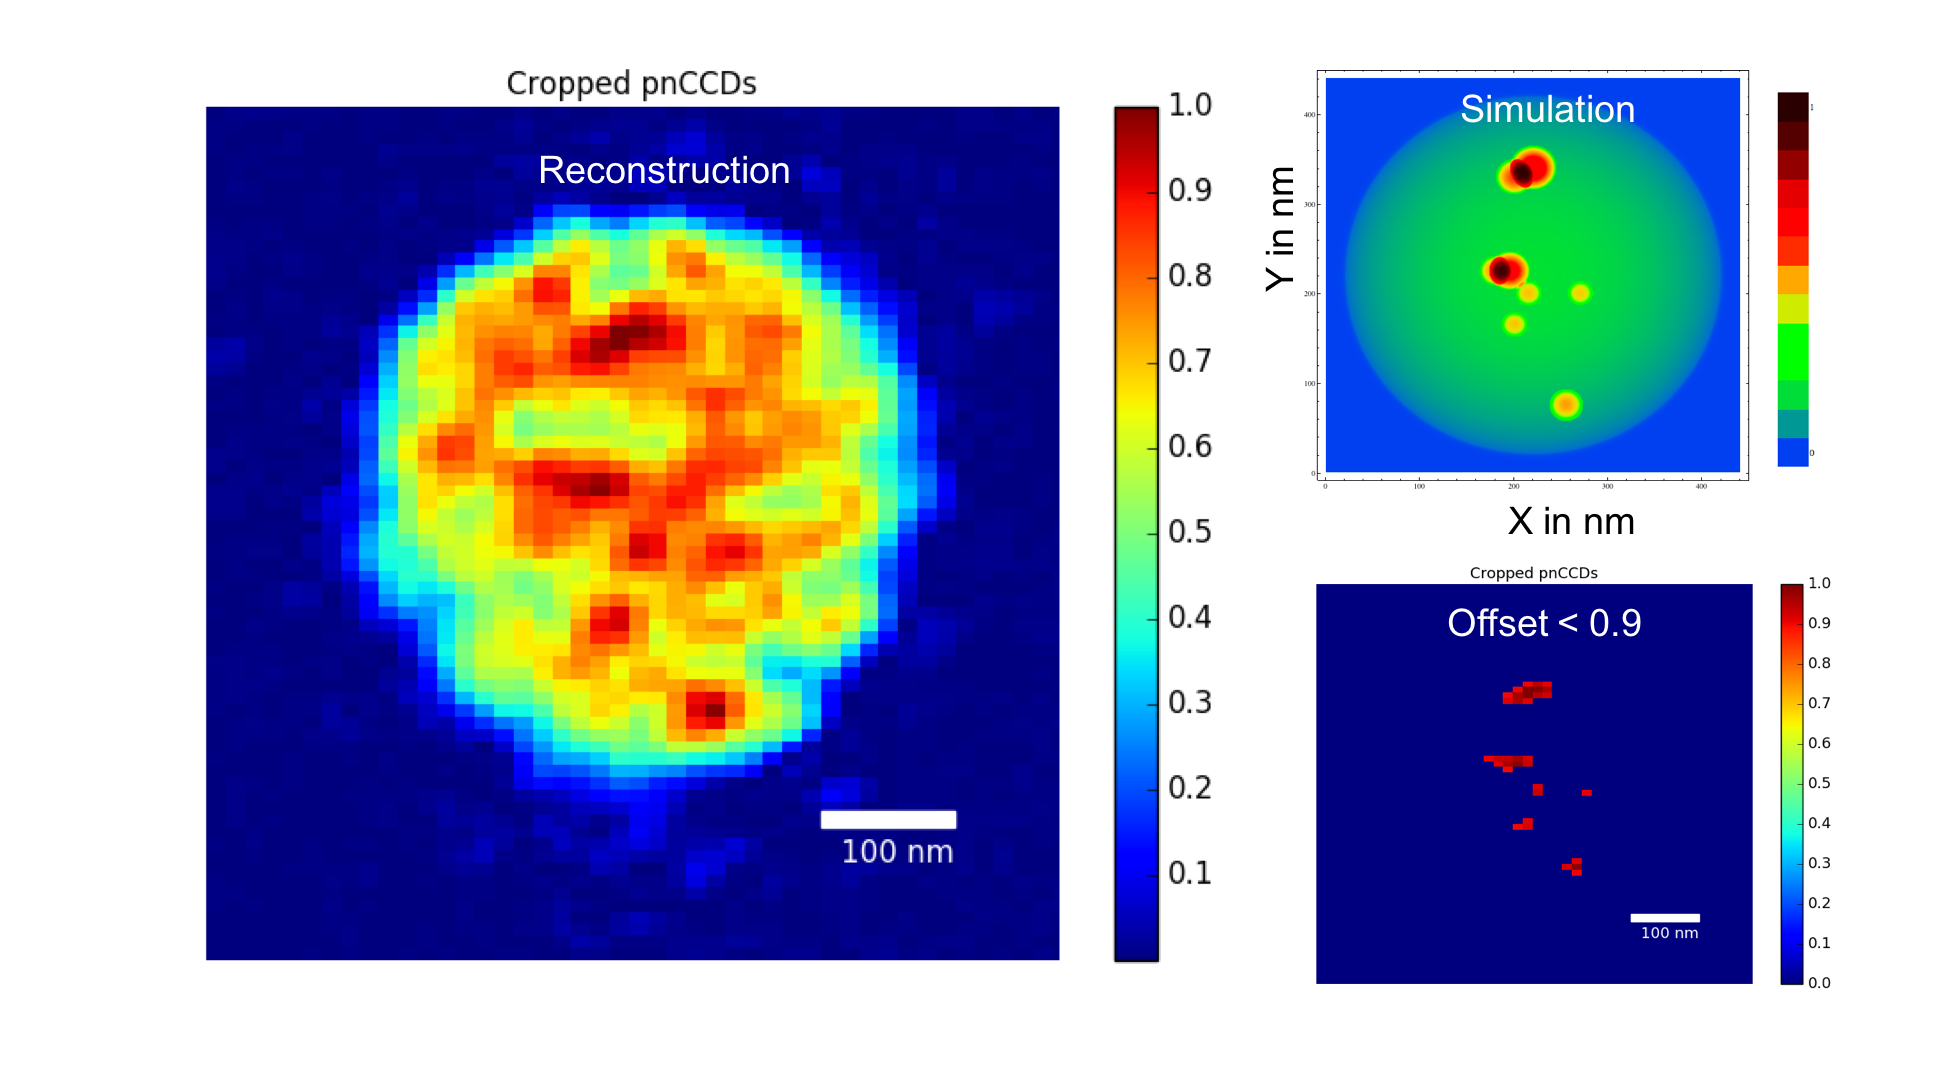
\includegraphics[width=0.80\textwidth]{images/results/reconstructions-to-simulations.png}
 	\caption{Real-space reconstruction of a HeXe-cluster that has a radius of $r\approx 210$ nm and a Xe-doping level of $\sim 0.5\%$ and corresponding simulation. The electron density indicates a Xe-cluster arrangement of the plum-pudding few scatterer case discussed in figure \ref{fig:HeXe-plum-pudding}. The largest Xe-cluster appear to be $\sim 50$ nm in diameter and should therefore be well resolved. The normalized intensity map can then be offset and mimicked by 2D electron density projections.}
 	\label{fig:HeXe-cluster-60}
\end{figure}
Coherent diffractive imaging is a direct structural measurement technique and allows us to investigate the actual arrangement within a HeXe-cluster. Figure \ref{fig:HeXe-cluster-60} shows a reconstruction of a HeXe-cluster that has a radius of $r\approx 210$ nm and a Xe-doping level of $\sim 0.5 \%$. The reconstruction indicates a plum-pudding arrangement, where a few Xe-cluster (intense, dark red spots) are randomly distributed within the He-droplet (less intense, green to orange area). The normalized intensity map from the reconstruction may be offset to guide the eye to dense centers. To move on, we may move the gained information from the reconstructions to reverse engineer the electron density and subsequently study the diffraction image in more detail. This is discussed in the next section and also a focus on the influence of radiation damage onto the diffraction pattern is set.
%
%
%
% \subsection{Diffraction images of helium cluster}
%%%%%%%%%%%%%%%%%%%%%%%%%%%%%%%%%%%%%%%
%- Work out radiation damage in 1D diffraction images.\\
%- Introduce envelope to show the radiation damage effect - important to compare to HeXe data.\\
%- Eventually subsection for reconstructions.
%%%%%%%%%%%%%%%%%%%%%%%%%%%%%%%%%%%%%%%
%
%
%
\section{Sacrificial tampered layers inhibit effects of radiation damage}\label{sec:helium-xenon-data}
%%%%%%%%%%%%%%%%%%%%%%%%%%%%%%%%%%%%%%
%-Presentation of HeXe data
%%%%%%%%%%%%%%%%%%%%%%%%%%%%%%%%%%%%%%
\begin{figure}
	\centering
		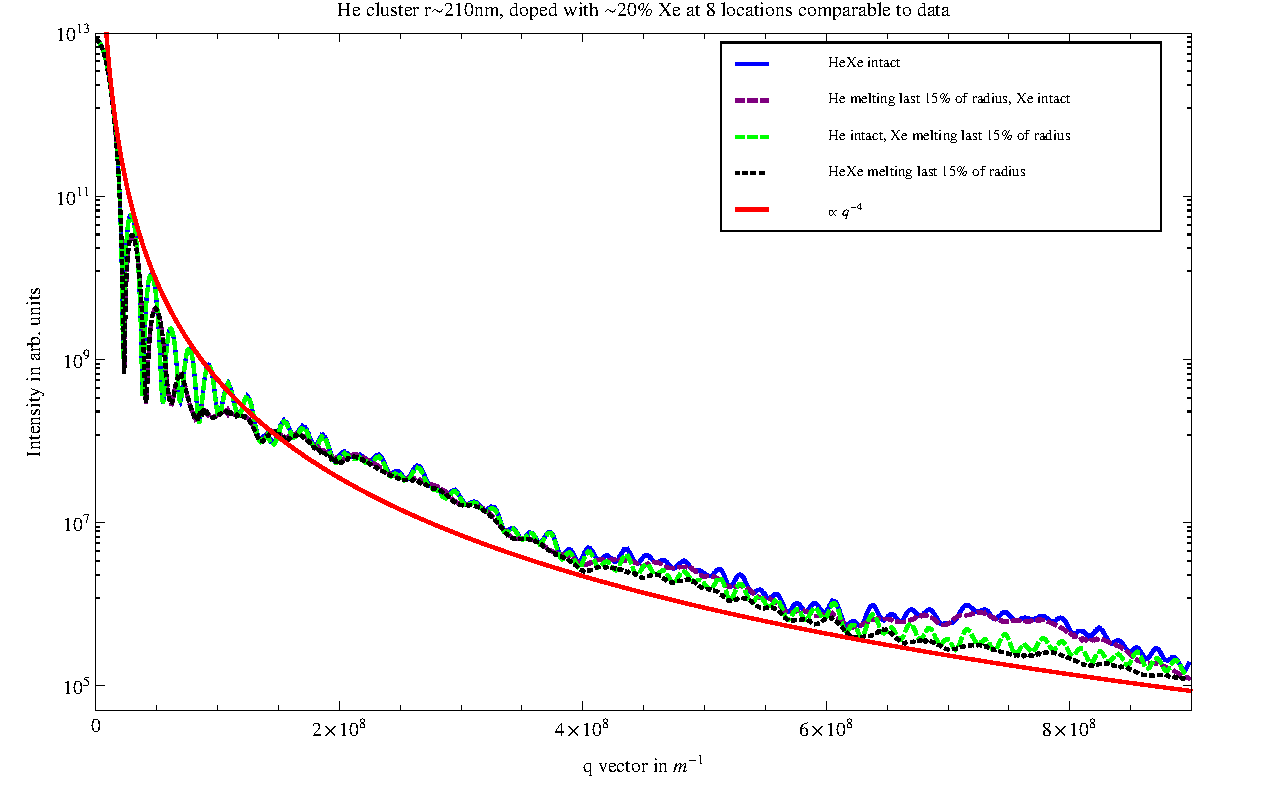
\includegraphics[width=1.00\textwidth]{images/results/simulations-damage-explain.pdf}
	\caption{caption}
	\label{fig:simulations-damage-explain}
\end{figure}
Figure \ref{fig:simulations-damage-explain} shows a diffraction pattern from the simulated plum-pudding type electron density shown in figure \ref{fig:HeXe-cluster-60} that illustrate radiation damage. As described in section \ref{sec:2d-simulations}, the radiation damage is simulated via an expansion of the outer layers of a sphere. The He-droplet has a radius $r_{\text{He}}=210$ nm and a strong Xe-doping of $\sim 20 \%$ to illustrate the effect. The blue, solid curve describes the scenario, where all spheres, i.e. clusters, are intact and no X-ray induced dynamics are present. The purple, dashed curve shows the case, where the last $15 \%$ in units of the He-droplet radius $r$ expand but leaving the Xe-cluster intact. Conversely, the green, dashed curve shows the effect, where the last $r\cdot 15 \%$ of the Xe-clusters expand but leaving the He-shell intact. Lastly, all spheres are expanding at $r\cdot 15 \%$. It can be clearly seen, that the expansion of each cluster type effects either low spatial frequencies when the He-droplet is expanding or high spatial frequencies when the (much smaller) Xe-cluster are expanding. At the vast size differences of the Xe-cluster $r_{\text{Xe}}=\{TBD\}$ allow a strict separation between the He-droplet, i.e. the shell, expanding, or the Xe-clusters, i.e. the cores.\\
%Now that we have discussed the effects of X-ray induced dynamics, i.e. radiation damage, in Xe-clusters by analyzing single-shot diffraction pattern and time-of-flight mass spectroscopy and also having understood the structure of heterogeneous HeXe cluster as they arrange in a \textit{plum-pudding} type model, where few Xe-scatterer are present in a large He-droplet, we can discuss the diffraction pattern from the pump--probe data of HeXe-clusters. Let us start off by reusing the 2D simulations, described in section \ref{sec:2d-simulations}, using damaged spheres to investigate the effects onto the diffraction pattern.\\
\begin{figure}
	\centering
		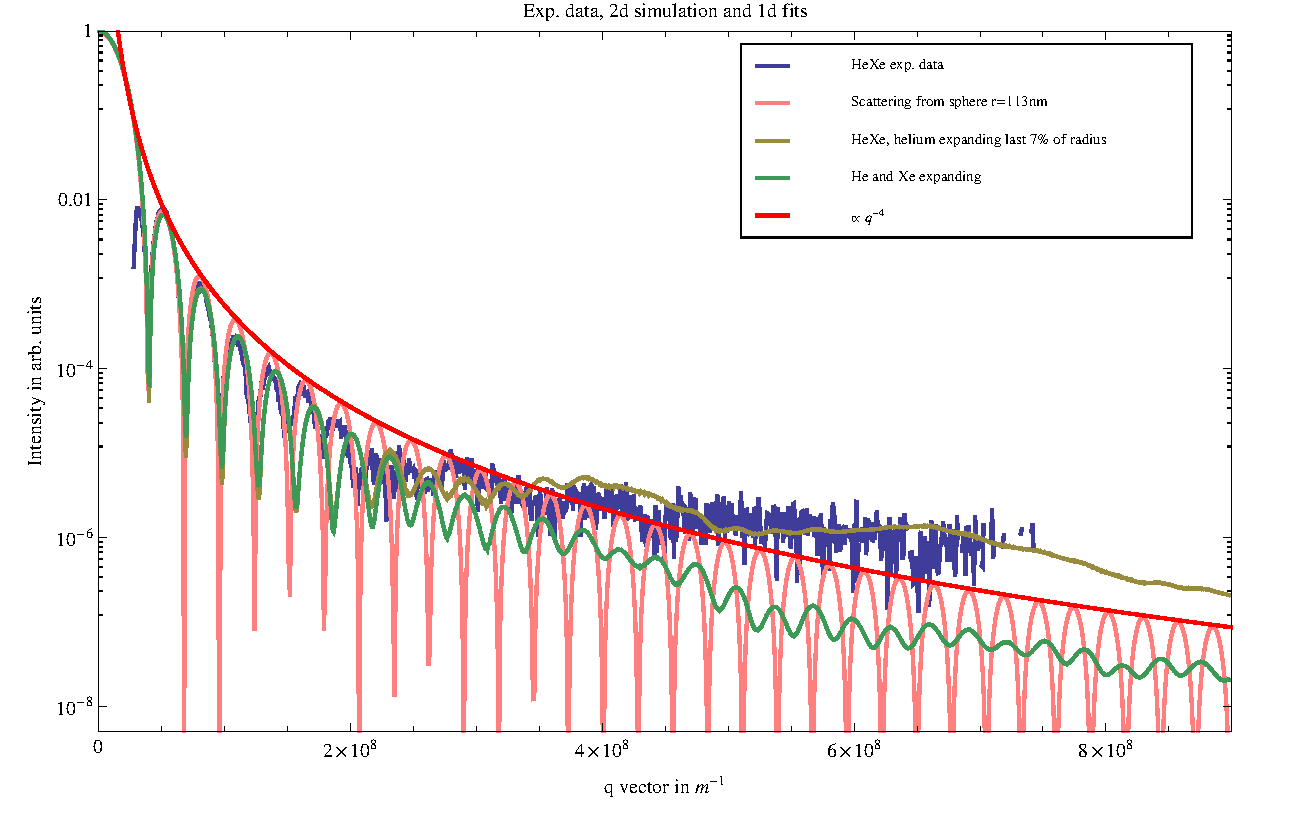
\includegraphics[width=1.00\textwidth]{images/results/HeXe-cluster-113-0-5-doping.pdf}
	\caption{caption}
	\label{fig:HeXe-cluster-113-0.5}
\end{figure}
We can use this insight to compare the 2D-simulations to the actual diffraction pattern. Figure \ref{fig:HeXe-cluster-113-0.5} shows a measured diffraction pattern at a time delay $\Delta t=800$ fs between pump and probe beam and a fit using the discussed 2D-simulations. The simulations were fitted using xenon doping levels from comparable other shots at zero delay. It can be assumed that the doping level is constant, as the doping unit parameter remain unchanged and the doping mostly depends on the size of the incoming He-droplet. To fit the data, the radius of the He-droplet was expanding as per XXX TBD \% and the Xe-cluster remained intact.\\
If we increase the doping, we can see that XXX
%
%
%
%\subsection{Time-of-flight data of helium-xenon core-shell systems}
%%%%%%%%%%%%%%%%%%%%%%%%%%%%%%%%%%%%%%%%%%%%%%%%%%%
%- Show dynamics of XeHe data in tof trace.\\
%- More hefty nanoplasma expansion in HeXe than in raw He.\\
%- Complement with simulations from Phay.
%%%%%%%%%%%%%%%%%%%%%%%%%%%%%%%%%%%%%%%%%%%%%%%%%%%
%
%
%
%\subsection{Diffraction images of helium-xenon core shell systems}
%%%%%%%%%%%%%%%%%%%%%%%%%%%%%%%%%%%%%%%%%%%%%%%%%
%- Discuss diffraction images\\
%- Show how scattering intensity drops from He signal but not from Xe signal.\\
%- Eventually subsection for reconstructions.
%%%%%%%%%%%%%%%%%%%%%%%%%%%%%%%%%%%%%%%%%%%%%%%%%
%
%
%
%\subsection{Core-shell system considerations}
%
%
%
%\section{Static data}\label{sec:static}
%%%%%%%%%%%%%%%%%%%%%%%%%%%%%%%%%%%%%%%%%%
%-Include in other studies? Or appendix?
%%%%%%%%%%%%%%%%%%%%%%%%%%%%%%%%%%%%%%%%%%%%
%
%
%
\section{Discussion and conclusion of the X-ray pump -- X-ray probe study}
%%%%%%%%%%%%%%%%%%%%%%%%%%%%%%%%%%%%%%%%
%- Conclusion where the results are compared to each other\\
%- This experiment shows that heterogeneous clusters, as in tampered layers, do inhibit radiation damage of the sample target while the sacrificial layer undergoes a rapid nanoplasma transition.
%%%%%%%%%%%%%%%%%%%%%%%%%%%%%%%%%%%%%%%%%%
The X-ray pump -- X-ray probe study reveals some induced dynamics in Xe- and HeXe-cluster. In pristine Xe-cluster, we observe the nanoplasma expansion in the diffraction patternsa nd we can compare the results to other pump--probe studies using optical pump laser. The absorbed energy by the Xe-cluster is comparable in the optical to X-ray study (TBD), which is most relevant for the extend of the nanoplasma expansion. The time-of-flight spectroscopy reveals a to optical laser hidden resonance that is likely due to relaxation processes in the highly excited atoms. As an inner shell electron is ionized a chemical shift changes the ionization potentials and dynamic relaxation processes allow the absorption of more photons at certain stages \citep{Ho-2014-PRL}.\\
Heterogeneous HeXe-cluster, doped using the pickup-principle, arrange in a plum-pudding type model, where Xe atoms form few Xe-cluster within one large (superfluid) He-droplet. 2D-simulations furthermore show that the X-ray induced dynamics in HeXe-cluster manifest only in the He-droplet.
%
%
%